% !TeX program = lualatex
% !TeX encoding = utf8
% !TeX spellcheck = uk_UA
% !TeX root =../ClassicalEletrodynamics.tex

%=========================================================
%\Opensolutionfile{answer}[\currfilebase/\currfilebase-Answers]
%\Writetofile{answer}{\protect\section*{\nameref*{\currfilebase}}}
\chapter{Величини, що спостерігаються в електродинаміці}\label{\currfilebase}
%=========================================================



%% --------------------------------------------------------
\section{Заряд, електричне та магнітне поле}
%% --------------------------------------------------------



Основними спостережуваними величинами в електродинаміці є
електричний заряд та електромагнітне поле --- сукупність електричного та
магнітного полів. Статичні заряди створюють електричне поле, рух зарядів
спричинює магнітне поле. Навпаки, електромагнітне поле створює силу, що діє
на заряджене тіло. Ця схема відповідає концепції близькодії, яка домінує в
сучасній фізиці; за цією концепцією заряди взаємодіють між собою через
електромагнітне поле, а не безпосередньо.

%% --------------------------------------------------------
\subsection*{Закон Кулона}
%% --------------------------------------------------------

Числову характеристику заряду можна дати, вимірюючи
силу взаємодії F між двома точковими нерухомими зарядами. Якщо ці заряди
розташовані на відстані R, за абсолютною величиною:
\begin{equation}\label{eq:Columb_low}
    F = k \frac{q_1q_2}{R^2},
\end{equation}
де $q_1$, $q_2$ --- заряди тіл, $k$ --- коефіцієнт пропорційності, що залежить від вибору
системи одиниць. Це співвідношення називають законом Кулона; воно
неодноразово перевірялося різними експериментальними методами. Сила, з
якою один заряд діє на інший, направлена вздовж лінії центрів зарядів.
З спостережень відомо, що існують лише два сорти електричних зарядів,
причому заряди однакового сорту завжди притягуються, а заряди різного сорту
— відштовхуються. Цю обставину враховуємо, вводячи знаки зарядів в
формулі~\eqref{eq:Columb_low}. Від'ємними вважаються заряди того ж сорту, що й заряд
електрона. Заряд є адитивною числовою величиною: заряд будь-якої
системи є алгебраїчною сумою зарядів його підсистем.

Формула~\eqref{eq:Columb_low} дає змогу визначити заряд й подати процедуру його
вимірювання (тобто спосіб порівняння заряду з деяким еталоном) за
допомогою вимірювання сили взаємодії. В гаусовiй системi одиниць два
одиничних заряди створюють силу взаємодiї $1\ \text{дина} = 1\ \text{г}\cdot\text{см} / \text{c}^2$,
якщо знаходяться на відстані $1$~см. Відповідно в~\eqref{eq:Columb_low} слід покласти $k=1$. Це --- означення
одиничного заряду в гаусовій системі (тут одиниця заряду не має спеціальної назви):
\begin{equation*}
    \left[q\right] = \text{г}^{1/2}\cdot\text{см}^{3/2}\cdot\text{с}^{-1}.
\end{equation*}

Підкреслимо, що в~\eqref{eq:Columb_low} йдеться про точкові сферичні заряди, тобто
такі, взаємодія яких не залежить від їх орієнтації. Справа в тому, що хоча
точкове тіло --- це таке, розмірами якого можна знехтувати, в конкретній задачі
розподіл зарядів всередині цього тіла може бути різко неоднорідним. Це
спричинюватиме, взагалі кажучи, відмінність сили взаємодії від~\eqref{eq:Columb_low}.
Прикладом може служити взаємодія точкових диполів. Далі під точковим
зарядом ми будемо розуміти саме сферичний точковий заряд, якщо немає
інших застережень.

%% --------------------------------------------------------
\subsection*{Напруженість електричного поля та індукція магнітного поля}
%% --------------------------------------------------------

 Числову характеристику електромагнітного поля можна дати,
вимірюючи сили, що діють на рухомий електричний пробний заряд. Пробний
заряд --- це такий, впливом якого на зовнішнє поле можна знехтувати.
 З експерименту відомо, що на заряджене точкове пробне тіло (сферичний
точковий заряд) в електромагнітному полі діє сила Лоренца:
\begin{equation}\label{eq:Lorentz_force}
    \vect{F} = q\left( \Efield + \frac1c \left[ \vect{v}\times\Bfield\right] \right),
\end{equation}
де $q$ --- заряд тіла що не залежить від швидкості, $\vect{v}$ --- його швидкість, а вектори $\Efield$
та $\Bfield$ не залежать від тіла і є характеристиками поля; коефіцієнт $c$ визначається системою одиниць.

Вектор $\Efield$ називають напруженістю електричного поля, $\Bfield$ --- індукцією
магнітного поля. Сукупність цих двох векторів, заданих в кожній точці
простору, повністю визначають стан електромагнітного поля в класичній
фізиці. Формула \eqref{eq:Lorentz_force} також дозволяє узагальнити процедуру визначення
заряду на випадок руху тіла. Адже спосіб, що базується на законі Кулона
\eqref{eq:Columb_low}, працює лише для нерухомих зарядів.
Спостерігаючи за рухом заряджених частинок, можна визначити (див. вправу \ref{prb:1}) напруженість електричного поля та індукцію магнітного поля.
Звичайно, на практиці існують більш зручні методи вимірювання $\Efield$ та $\Bfield$.

%=========================================================
\begin{problem}\label{prb:1}%
Нехай в експерименті визначають прискорення в однорідному
електромагнітному полі електронів з заданими початковими швидкостями.
Покажіть, що це дає змогу однозначно визначити вектори $\Efield$
та $\Bfield$ за формулою~\eqref{eq:Lorentz_force}.
\end{problem}

В гаусовій системі одиниць коефіцієнт $с = 2,9979⋅1010$~см/с --- швидкість
світла, тому розмірності $\Efield$
та $\Bfield$ формально однакові:
\begin{equation*}
    \left[ E\right]  = \left[ B \right]  = \text{г}^{1/2}\cdot\text{см}^{-1/2}\cdot\text{с}^{-1}.
\end{equation*}
Одиниця магнітної індукції має назву <<Гаусс>>. Її не застосовують у випадку
електричного поля, хоча формально його напруженість має цю ж розмірність.


%% --------------------------------------------------------
\section{Основні властивості зарядів та електромагнітного поля}
%% --------------------------------------------------------

%% --------------------------------------------------------
\subsection*{Принцип суперпозиції}
%% --------------------------------------------------------

Формула~\eqref{eq:Lorentz_force} дає змогу виміряти
електромагнітне поле, вивчаючи його вплив на рух точкового заряду, але не
дозволяє його розрахувати, виходячи з розподілу зарядів. Для цього потрібні

рівняння, що пов’язують певним чином електромагнітне поле з його
джерелами. Але перш ніж записати ці рівняння, відзначимо фундаментальний
принцип суперпозиції електромагнітних полів: напруженість електричного
поля $\Efield$ та індукція $\Bfield$ магнітного поля, створюваних системою зарядів, є сумою
полів $\Efield_k$ , $\Bfield_k$, що створюються окремими зарядами (або підсистемами) цієї
системи:
\begin{equation}
    \Efield = \sum\limits_k \Efield_k, \quad \Bfield = \sum\limits_k \Bfield_k.
\end{equation}
 Тут поле $(\Efield_k, \Bfield_k)$ $k$-ї підсистеми розглядається окремо.
 Це твердження, яке значно спрощує розв’язання задач електродинаміки,
випливає з дослідних даних. Взагалі кажучи, можна навести приклади, коли
фізичні поля не задовольняють принципу суперпозиції. Але ці явища класична
електродинаміка не розглядає. В звичайних умовах принцип суперпозиції
виконується з дуже високою точністю. Принцип суперпозиції тісно пов’язаний
з адитивністю заряду.


%% --------------------------------------------------------
\subsection*{Квантування (дискретність) електричного заряду}
%% --------------------------------------------------------


З експериментів відомо, що найменшим відомим зарядом є заряд електрона, що наближено дорівнює (за абсолютною величиною) $е=4,8\cdot10^{-10}$ одиниць
гаусової системи. Заряд електрона є від’ємним; заряд протона – додатній і дорівнює заряду електрона з оберненим знаком. Будь-які заряди, що
спостерігалися, кратні заряду електрона. Пошуки вільних зарядів, менших за е, або не кратних цій величині, дали негативний результат. Зауважимо, що
відхилення зарядів протона й електрона призвело б до порушення електронейтральності атомів, що суперечить експериментальним даним. Слід відзначити, що
сучасні експерименти дають змогу вивчати розподіл заряду всередині елементарних часток. Але наявність неперервного розподілу густини заряду всередині,
наприклад, протона чи нейтрона, яка досліджується при зіткненнях елементарних часток, не суперечить квантуванню електричного заряду. Ця властивість
стосується повного заряду частинок, що можуть існувати iзoльовано від інших.

%% --------------------------------------------------------
\subsection*{Інваріантність електричного заряду}
%% --------------------------------------------------------


Величина заряду не залежить від
його швидкості відносно спостерігача. Неінваріантність заряду також могла б
призвести до порушення електронейтральності атомів, оскільки електрони в
атомах рухаються з швидкостями до 0,1 с; величина швидкості електронів
різна на різних оболонках і відрізняється в різних атомах.


%% --------------------------------------------------------
\subsection*{Збереження електричного заряду}
%% --------------------------------------------------------


Якщо вважати встановленим факт
квантування заряду, то збереження заряду в звичайних умовах пов’язано зі
збереженням кількості протонів та електронів в атомах. Однак відомо, що
електричний заряд зберігається і тоді, коли мають місце взаємоперетворення
елементарних часток.

Область застосовності законів збереження, квантування та інваріантності
електричного заряду виходить далеко за рамки класичної електродинаміки. На
цей час порушення цих законів невідомі.


%% --------------------------------------------------------
\section{Розподіли зарядів та струмів}
%% --------------------------------------------------------


%% --------------------------------------------------------
\subsection*{Сила струму}
%% --------------------------------------------------------


Дамо числову характеристику електричного струму --- впорядкованого руху носіїв заряду.
Нехай поверхня $S$ є орієнтованою, тобто визначений певний додатній
напрямок перетину цієї поверхні. Нехай $q(t)$ --- сумарний заряд, що перетнув $S$ з
урахуванням напрямку за час t з початку відліку. Тоді, за визначенням, сила
струму через поверхню $S$ (в додатному напрямку) є:
\begin{equation}\label{eq:I_S}
    I_S(t) = \frac{dq(t)}{dt}.
\end{equation}

У разі сталого струму --- це заряд, що перетинає $S$ за одиницю часу.


\begin{itemize}
\item  Здавалося б, що запис \eqref{eq:I_S} не є цілком коректний, оскільки заряди дискретні і $q(t)$ змінюється стрибками. Однак завдяки малості цих
стрибків $q(t)$ можна апроксимувати гладкою функцією, що є цілком правомірно в макроскопічних застосуваннях.
\item  Необхідними елементами визначення сили струму є поверхня $S$ та її орієнтація. Але якщо йдеться про сталий струм в провідникові, форма перерізу,
через який обчислюється струм, не є суттєвою. Завдяки закону збереження заряду струм через $S_1$, $S_2$ та $S_3$ (див. рис.~\ref{tikz:current})
однаковий. Адже у
разі супротивного заряд з часом міг би накопичуватися, наприклад, між $S_1$ та $S_2$, що суперечило б умові стаціонарності.
\end{itemize}

%---------------------------------------------------------
\begin{SCfigure}[1][h!]
    \centering
    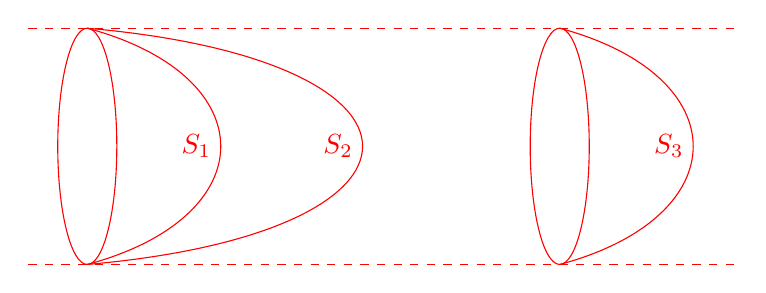
\begin{tikzpicture}[scale=1.5]
        \def\R{1}
        \draw[red, dashed] (0, {+\R}) -- ++(6, 0);
        \draw[red, dashed] (0, {-\R}) -- ++(6, 0);
        \draw[red] (0.5, 0) circle (0.25 and \R);
        \draw[red] (0.5, {+\R}) to[out=-15, in=15, looseness=2] node[pos=0.5, left] {$S_1$} (0.5, {-\R}) ;
        \draw[red] (0.5, {+\R}) to[out=-5, in=5, looseness=4] node[pos=0.5, left] {$S_2$} (0.5, {-\R}) ;

        \draw[red] (4.5, 0) circle (0.25 and \R);
        \draw[red] (4.5, {+\R}) to[out=-15, in=15, looseness=2] node[pos=0.5, left] {$S_3$} (4.5, {-\R}) ;
    \end{tikzpicture}
\caption{}
\label{tikz:current}
\end{SCfigure}
%---------------------------------------------------------


%% --------------------------------------------------------
\subsection*{Мікроскопічний та макроскопічний підхід в електродинаміці}
%% --------------------------------------------------------



Мікроскопічний підхід оперує з якомога точними значеннями величин, що характеризують електромагнітні взаємодії з врахуванням будови речовини і в цьому
розумінні він є найбільш повним та послідовним. Але використання мікроскопічного підходу не завжди доцільно. Приклад такої ситуації – попереднє
обговорення формули~\eqref{eq:I_S}). У макроскопічних вимірюваннях амперметр вимірює усереднене значення сили струму, і тут можна не зважати на
дискретну будову електрики. Це дає змогу застосовувати відповідну математичну модель процесу вимірювання, яка працює з гладкими функціями $I_S(t)$ та
$q(t)$ в~\eqref{eq:I_S}). Якщо треба охарактеризувати нерівномірність розподілу зарядів в об’ємі, можна також використовувати ідеалізацію, коли
вводиться густина заряду, яка є неперервною функцією координат. Це можливо, якщо кожна ділянка цього об’єму, де виконують вимірювання, містить досить
велику кількість елементарних зарядів. Далі під макроскопічними величинами будемо розуміти такі, що отримані внаслідок деякого усереднення --- за часом
або у деяких просторових масштабах. З одного боку макроскопічний підхід пов’язаний з можливостями конкретного фізичного експерименту, в якому
мікробудова може бути несуттєвою, з іншого боку, застосування неперервних розподілів дає змогу застосувати апарат математичного аналізу для опису явищ.



%% --------------------------------------------------------
\subsection*{Густина заряду}
%% --------------------------------------------------------


Для опису заданого просторового розподілу заряду
введемо функцію ρ, що може залежати від координат та від часу і дозволяє
обчислити заряд в будь-якій області $\Omega$ за формулою:
\begin{equation}\label{eq:q}
    q_{\Omega} = \iiint\limits_{\Omega} \rho(t, \vect{r}) dV
\end{equation}
де $\vect{r} = x\vect{e}_x + y\vect{e}_y + z\vect{e}_z$, $dV=dx\ dy\ dz$.

Інакше, елемент заряду в об’ємі $dV$ --- це є $dq = \rho(t, \vect{r}) dV$.

Функцію $\rho(t, \vect{r})$ називають густиною заряду. Для сталого розподілу це є
величина заряду в одиниці об’єму.

Якщо в середовищі присутні однакові носії з зарядом $q$ й об’ємною
густиною їх числа (концентрацією) $n$:
\begin{equation}
    \rho = qn
\end{equation}
а в більш загальному випадку:
\begin{equation}
    \rho(t, \vect{r}) = \sum\limits_k q_kn_k(t, \vect{r}),
\end{equation}
де індекс $k$ відповідає різним сортам носіїв заряду, кожен із своєю концентрацією.


%% --------------------------------------------------------
\subsection*{Густина струму}
%% --------------------------------------------------------


Цю величину можна визначити формулою для сили
струму через поверхню $S$:
\begin{equation}
    I_S(t) = \iint\limits_S \vect{j}(t, \vect{r})\cdot d\vect{S},
\end{equation}
де $\vect{j}$ --- вектор густини струму, що не залежить від $S$, $d\vect{S} = \vect{n} dS$, $\vect{n}$ --- нормаль до
елемента поверхні $dS$. Густина сили струму дає напрям руху зарядів в даному
елементі об’єму і за абсолютною величиною --- силу струму через одиничний
переріз, проведений перпендикулярно до цього напрямку. Маємо:
\begin{equation}
    \vect{j} = nq\vect{v}
\end{equation}
якщо усі заряди з концентрацією $n$ мають однакову швидкість $\vect{v}$ та заряд $q$,
або для декількох сортів носіїв заряду:
\begin{equation}
\vect{j} = \sum\limits_k q_k n_k\vect{v}_k
\end{equation}
Ще більш загальний вираз можна записати за наявності розподілу за
швидкостями:
\begin{equation}
\vect{j} = \sum\limits_k \int  q_k f_k(t, \vect{r}, \vect{v}) \vect{v}_k dV_xdV_ydV_z,
\end{equation}
де $f_k(t, \vect{r}, \vect{v})$ --- функція розподілу k–го сорту зарядів за швидкостями.


%% --------------------------------------------------------
\subsection*{Поверхневі заряди та струми}
%% --------------------------------------------------------


 Якщо електричні заряди зосереджені у
тонкому прошарку поблизу деякої поверхні, доцільно ввести поверхневу
густину заряду σ. Аналогічно \eqref{eq:q}, покладемо:
\begin{equation}
    q_S(t) = \iint\limits_S \sigma(t, \xi, \eta) dS(\xi, \eta).
\end{equation}
де $q_S$ --- заряд на ділянці S цієї поверхні, $\xi$ та $\eta$ --- координати на поверхні; $\sigma$
характеризує вміст заряду на одиниці площі.


%---------------------------------------------------------
\begin{SCfigure}[2][h!]
    \centering
    \begin{tikzpicture}[scale=1.5]
        \draw[midarrow, tangent=0.2, tangent=0.4, tangent=0.6, tangent=0.8, red, thick] (-1, 1) node[above, text=red] {$L$} to[out=-90, in=115] (0, -1) ;
        \foreach \i in {1,...,4}{
            \draw[->, use tangent=\i, blue] (0,0) coordinate (T\i)-- ++(90:0.5);
            \draw[->] (T\i) -- ++(1, 0);
            \draw[] (T\i) -- ++(-1, 0);
        }
    \end{tikzpicture}
\caption{}
\label{surface_current}
\end{SCfigure}
%---------------------------------------------------------

 За наявності руху поверхневих зарядів визначимо силу струму через лінію
$L$ (див. рис.~\ref{surface_current}) на цій поверхні:
\begin{equation}
    I_L(t) = \frac{dq_L(t)}{dt},
\end{equation}
де $dq_L$ --- заряд, що перетинає $L$ за час $ t$ з початку спостереження. Тут також
має бути зафіксований додатній напрямок при перетині L вздовж цієї поверхні.
Лінійна густина i поверхневого струму визначається формулою (для будьякої лінії $L$ на поверхні):
\begin{equation}
    I_L(t) = \int\limits_L \vect{i}(t, \xi, \eta) d\vect{l}(\xi, \eta),
\end{equation}
де $d\vect{l} = \vect{n} d \ell$ --- орієнтовний елемент довжини на $L$, $\vect{n}$ --- нормаль до $L$ на поверхні у
точці інтегрування.



%% --------------------------------------------------------
\section{Математичний запис закону збереження заряду}
%% --------------------------------------------------------


Нехай $q_{\Omega}$ --- заряд в деякому об'ємi $\Omega$, $\partial\Omega$ --- поверхня, що обмежує цей
об'єм, $I_{\partial\Omega}$ --- струм, що виходить через $\partial\Omega$ назовні з об'єму $\Omega$ (будемо вважати,
що це відповідає додатній орiєнтацiї поверхнi $\Omega$). Тоді, за законом збереження заряду i за означенням струму~\eqref{eq:I_S}, маємо у кожний момент
часу:
\begin{equation}\label{eq:charge_conservation_low_int}
    \frac{dq_{\Omega}}{dt} + I_{\partial\Omega}   = 0.
\end{equation}

Спiввiдношення \eqref{eq:charge_conservation_low_int} є інтегральною формою закону збереження
заряду. Для поверхневих зарядів та струмів можна подати аналогічне
співвідношення, що пов’язує швидкість зміни заряду на дiлянку поверхнi та
струм через межу цiєї дiлянки.

Отримаємо з \eqref{eq:charge_conservation_low_int} диференціальне спiввiдношення для густини заряду
$\rho(t, \vect{r})$ та густини об'ємного струму $\vect{j}(t, \vect{r})$ . Використовуючи визначення \eqref{eq:q}
для нерухомого об'єму:
\begin{equation*}
    \frac{dq_{\Omega}}{dt} = \frac{d}{dt} \iiint\limits_{\Omega} \rho(t, \vect{r}) dV = \iiint\limits_{\Omega} \frac{\partial\rho(t, \vect{r})}{\partial
    t} dV.
\end{equation*}

Тодi з \eqref{eq:charge_conservation_low_int}  та за виначенням густини струму \eqref{eq:I_S}:
\begin{equation*}
    \iiint\limits_{\Omega} \frac{\partial\rho(t, \vect{r})}{\partial
    t} dV + \iint\limits_{\partial\Omega} \vect{j}\cdot d\vect{S} = 0.
\end{equation*}
Перетворимо iнтеграл по замкненiй поверхнi $\partial\Omega$, що оточує об'єм $\Omega$, за
теоремою Остроградського-Гаусcа:
\begin{equation*}
    \iint\limits_{\partial\Omega} \vect{j}\cdot d\vect{S} = \iiint\limits_{\Omega}\Div\vect{j} dV,
\end{equation*}
звідки
\begin{equation*}
    \iiint\limits_{\Omega} \left(\frac{\partial\rho(t, \vect{r})}{\partial
    t}  +  \Div\vect{j} \right) dV =0.
\end{equation*}

Це співвідношення виконується для будь-якого об'єму $\Omega$, тому
підінтегральний вираз має дорівнювати нулю:
\begin{equation}\label{eq:charge_conservation_low_diff}
    \frac{\partial\rho(t, \vect{r})}{\partial t}  +  \Div\vect{j}  = 0
\end{equation}

Це диференцiальна форма закону збереження заряду або рівняння неперервності для об’ємної густини зарядів.

%\Closesolutionfile{answer}

